\documentclass[table]{beamer}
%[]中可以使用draft、handout、screen、transparency、trancompress、compress等参数

%指定beamer的模式与主题
\mode<presentation>
{
  \usetheme{Madrid}
%\usetheme{Boadilla}
%\usecolortheme{default}
%\usecolortheme{orchid}
%\usecolortheme{whale}
%\usefonttheme{professionalfonts}
}

%\usetheme{Madrid}
%这里还可以选择别的主题:Bergen, Boadilla, Madrid, AnnArbor, CambridgeUS, Pittsburgh, Rochester, Warsaw, ...
%有导航栏的Antibes, JuanLesPins, Montpellier, ...
%有内容的Berkeley, PaloAlto, Goettingen, Marburg, Hannover, ...
%有最小导航栏的Berlin, Ilmenau, Dresden, Darmstadt, Frankfurt, Singapore, Szeged, ...
%有章和节表单的Copenhagen, Luebeck, Malmoe, Warsaw, ...

%\usecolortheme{default}
%设置内部颜色主题(这些主题一般改变block里的颜色);这个主题一般选择动物来命名
%这里还可以选择别的颜色主题,如默认的和有特别目的的颜色主题default,structure,sidebartab,全颜色主题albatross,beetle,crane,dove,fly,seagull,wolverine,beaver

%\usecolortheme{orchid}
%设置外部颜色主题(这些主题一般改变title里的颜色);这个主题一般选择植物来命名
%这里还可以选择别的颜色主题,如默认的和有特别目的的颜色主题lily,orchid,rose

%\usecolortheme{whale}
%设置字体主题;这个主题一般选择海洋动物来命名
%这里还可以选择别的颜色主题,如默认的和有特别目的的颜色主题whale,seahorse,dolphin

%\usefonttheme{professionalfonts}
%类似的还可以定义structurebold,structuresmallcapsserif,professionalfonts

% 控制 beamer 的风格,可以根据自己的爱好修改
%\usepackage{beamerthemesplit} %使用 split 风格
%\usepackage{beamerthemeshadow} %使用 shadow 风格
%\usepackage[width=2cm,dark,tab]{beamerthemesidebar}

%插入音标
%\usepackage{tipa}
%\AtBeginDocument{
  %\renewcommand\textipa{\fontencoding{T3}\selectfont}
%}
%\AtBeginDocument{
  %\renewcommand\textipa[2][r]{{\fontfamily{cm#1}\tipaencoding #2}}
%}
%\renewenvironment{IPA}[1][r]
 %{\fontfamily{cm#1}\tipaencoding}
 %{}

% 设定英文字体
%\usepackage{fontspec}
% Fix bugs for fontspec in TeXLive2015
\ifdefined\suppressfontnotfounderror
  \expandafter\let\csname xetex_suppressfontnotfounderror:D\endcsname
    \suppressfontnotfounderror
\else
  \expandafter\let\csname xetex_suppressfontnotfounderror:D\endcsname
    \luatexsuppressfontnotfounderror
\fi
\usepackage[no-math]{fontspec}
\setmainfont{Times New Roman}
\setsansfont{Arial}
\setmonofont{Courier New}

% 设定中文字体
\usepackage[BoldFont,SlantFont,CJKchecksingle,CJKnumber]{xeCJK}
%\setCJKmainfont[BoldFont={Adobe Heiti Std},ItalicFont={Adobe Kaiti Std}]{Adobe Song Std}
\setCJKmainfont[BoldFont={Adobe Heiti Std},ItalicFont={Adobe Kaiti Std}]{WenQuanYi Micro Hei}
\setCJKsansfont{Adobe Heiti Std}
\setCJKmonofont{Adobe Fangsong Std}
\punctstyle{hangmobanjiao}

\defaultfontfeatures{Mapping=tex-text}
\usepackage{xunicode}
\usepackage{xltxtra}

\XeTeXlinebreaklocale "zh"
\XeTeXlinebreakskip = 0pt plus 1pt minus 0.1pt

\usepackage{setspace}
\usepackage{colortbl,xcolor}
\usepackage{hyperref}
%\hypersetup{xetex,bookmarksnumbered=true,bookmarksopen=true,pdfborder=1,breaklinks,colorlinks,linkcolor=blue,filecolor=black,urlcolor=cyan,citecolor=green}
\hypersetup{xetex,bookmarksnumbered=true,bookmarksopen=true,pdfborder=1,breaklinks,colorlinks,linkcolor=cyan,filecolor=black,urlcolor=blue,citecolor=green}

% 插入图片
\usepackage{graphicx}
\graphicspath{{figures/}}
% 图文混排
%\usepackage{picins}
\usepackage{floatflt}

% 可能用到的包
\usepackage{amsmath,amssymb}
%插入多媒体
%\usepackage{media9}
%\usepackage{movie15}
\usepackage{multimedia}
\usepackage{multicol}
\usepackage{multirow}

% 定义一些自选的模板,包括背景、图标、导航条和页脚等,修改要慎重
% 设置背景渐变由10%的红变成10%的结构颜色
%\beamertemplateshadingbackground{red!10}{structure!10}
%\beamertemplatesolidbackgroundcolor{white!90!blue}
% 使所有隐藏的文本完全透明、动态,而且动态的范围很小
\beamertemplatetransparentcovereddynamic
% 使itemize环境中变成小球,这是一种视觉效果
\beamertemplateballitem
% 为所有已编号的部分设置一个章节目录,并且编号显示成小球
\beamertemplatenumberedballsectiontoc
% 将每一页的要素的要素名设成加粗字体
\beamertemplateboldpartpage

% item逐步显示时,使已经出现的item、正在显示的item、将要出现的item呈现不同颜色
\def\hilite<#1>{
 \temporal<#1>{\color{gray}}{\color{blue}}
    {\color{blue!25}}
}

\renewcommand{\today}{\number\year 年 \number\month 月 \number\day 日}

%五角星
\usepackage{MnSymbol}

%去除图表标题中的figure等
\usepackage{caption}
\captionsetup{labelformat=empty,labelsep=none}

\usepackage{tabu}
\usepackage{multirow}
%表格自动换行
\usepackage{tabularx} 

% 千分号
%\usepackage{textcomp}

%罗马数字
\makeatletter
\newcommand{\rmnum}[1]{\romannumeral #1}
\newcommand{\Rmnum}[1]{\expandafter\@slowromancap\romannumeral #1@}
\makeatother

%分栏
\usepackage{multicol}

%\usepackage{enumitem}
%\usepackage{enumerate}

%键盘
\usepackage{keystroke}

%心形
%\usepackage{fdsymbol}

%插入源代码
\usepackage{listings}
\lstset{
  language=perl,                  % 程序语言名称:TeX, Perl, R, sh, bash, Awk
  basicstyle=\normalsize\tt,      %\tt指monospace字体族,程序源代码使用此族字体表示更加美观
  numbers=left,                   % 行号位置(左侧)
  numberstyle=\small,             % 行号字体的字号
  stepnumber=1,                   % 行号的显示步长
  numbersep=5pt,                  % 行号与代码间距
  backgroundcolor=\color{white},  % 背景色;需要 \usepackage{color}
  showspaces=false,               % 不显示空格
  showstringspaces=false,         % 不显示代码字符串中的空格标记
  showtabs=false,                 % 不显示 TAB
  tabsize=4, 
  frame=shadowbox,                % 把代码用带有阴影的框圈起来
  captionpos=b,                   % 标题位置
  breaklines=true,                % 对过长的代码自动断行
  breakatwhitespace=false,        % 断行只在空格处
  extendedchars=false,            % 解决代码跨页时,章节标题,页眉等汉字不显示的问题
  %escapeinside={\%*}{*},         % 跳脱字符,添加注释,暂时离开 listings 
  %escapeinside=``,
  commentstyle=\color{red!50!green!50!blue!50}\tt,  %浅灰色的注释
  rulesepcolor=\color{red!20!green!20!blue!20},     %代码块边框为淡青色
  keywordstyle=\color{blue!70}\bfseries\tt,         %代码关键字的颜色为蓝色,粗体
  identifierstyle=\tt,
  stringstyle=\tt,                % 代码字符串的特殊格式
  keepspaces=true,
  breakindent=1em,
  %breakindent=22pt,
  %breakindent=4em,
  breakautoindent=true,
  flexiblecolumns=true,
  aboveskip=1em,                  %代码块边框
  xleftmargin=2em,
  xrightmargin=2em
}

%\setbeamercolor{alerted text}{fg=magenta}
\setbeamercolor{bgcolor}{fg=yellow,bg=cyan}
%\setbeamercolor{itemize/enumerate body}{fg=green}

\begin{document}

%\includeonlyframes{current}

\logo{
\includegraphics[height=0.08\textwidth]{qr.png}}

% 在每个Section前都会加入的Frame
\AtBeginSection[]
{
  \begin{frame}<beamer>
    %\frametitle{Outline}
    \frametitle{教学提纲}
    \setcounter{tocdepth}{3}
    \begin{multicols}{2}
      \tableofcontents[currentsection,currentsubsection]
      %\tableofcontents[currentsection]
    \end{multicols}
  \end{frame}
}
% 在每个Subsection前都会加入的Frame
\AtBeginSubsection[]
{
  \begin{frame}<beamer>
%%\begin{frame}<handout:0>
%% handout:0 表示只在手稿中出现
    \frametitle{教学提纲}
    \setcounter{tocdepth}{3}
    \begin{multicols}{2}
    \tableofcontents[currentsection,currentsubsection]
    \end{multicols}
%% 显示在目录中加亮的当前章节
  \end{frame}
}

% 为当前幻灯片设置背景
%{
%\usebackgroundtemplate{
%\vbox to \paperheight{\vfil\hbox to
%\paperwidth{\hfil\includegraphics[width=2in]{tijmu_charcoal.png}\hfil}\vfil}
%}
\begin{frame}[plain]
  \begin{center}
    {\Huge 故事中的统计学\\}
    \vspace{1cm}
    {\LARGE 天津医科大学\\}
    %\vspace{0.2cm}
    {\LARGE 生物医学工程与技术学院\\}
    \vspace{1cm}
    {\large 2017-2018学年下学期(春)\\ 公共选修课}
  \end{center}
\end{frame}
%}



%\includeonlyframes{current}

\title[案例集锦与数据反驳]{第六章\quad 案例集锦与数据反驳}
\author[Yixf]{伊现富(Yi Xianfu)}
\institute[TIJMU]{天津医科大学(TIJMU)\\ 生物医学工程与技术学院}
\date{2018年4月}

\begin{frame}
  \titlepage
\end{frame}

\begin{frame}[plain,label=current]
  \frametitle{教学提纲}
  \setcounter{tocdepth}{3}
  \begin{multicols}{2}
    \tableofcontents
  \end{multicols}
\end{frame}


\section{回顾与拓展}
\subsection{回顾}
\begin{frame}
  \frametitle{回顾 | 太极拳}
  \begin{block}{太极拳健身}
打太极拳可以强壮身体,延长寿命,也就是说,打太极拳对身体健康有因果作用。但是打太极拳的人的寿命可能会与不打太极拳的人的寿命没有什么差异(或者反而打太极拳的人的寿命更短一些)。
  \end{block}
  \pause \pause \pause \pause
  \begin{block}{解析}
    可能是因为打太极拳的人都是体弱多病的人。
  \end{block}
\end{frame}

\begin{frame}
  \frametitle{回顾 | 铀矿工人}
  \begin{block}{矿工寿命}
    在铀矿工作的工人与其他人的寿命一样长(或更长),这并不能说明暴露于铀矿不会影响寿命。
  \end{block}
  \pause \pause \pause \pause
  \begin{block}{解析}
    可能是因为铀矿工人是经过挑选出来的身体健壮的人,假若当年他们不暴露于铀矿的话,寿命可能会更长一些。
  \end{block}
\end{frame}

\begin{frame}
  \frametitle{回顾 | 健康员工效应}
  \begin{block}{健康员工效应}
    有时在同一环境下,两组样本并不能直接进行比较。
  \end{block}
  \pause
  \begin{block}{实验}
假设将一组上班族与一组宇航员的健康状态进行比较研究。如果研究显示,两组没有显著差异,健康状况与工作环境之间没有相关性,我们是否就可以得出一个结论:在太空居住和工作不会给宇航员带来长期的健康风险?
  \end{block}
  \pause \pause \pause \pause
  \begin{block}{解析}
答案是不能。因为两组研究对象并没有站在同一起跑线上:宇航员团队会在申请者中挑选健康状况良好的候选人,然后按照一套综合的健康养生法进行保养,以便提前帮助宇航员克服微重力对生活带来的影响。
  \end{block}
\end{frame}

\subsection{拓展}
\begin{frame}
  \frametitle{拓展 | 四口之家的财富绝不会正好是两口之家的两倍}
  \begin{figure}
    \centering
    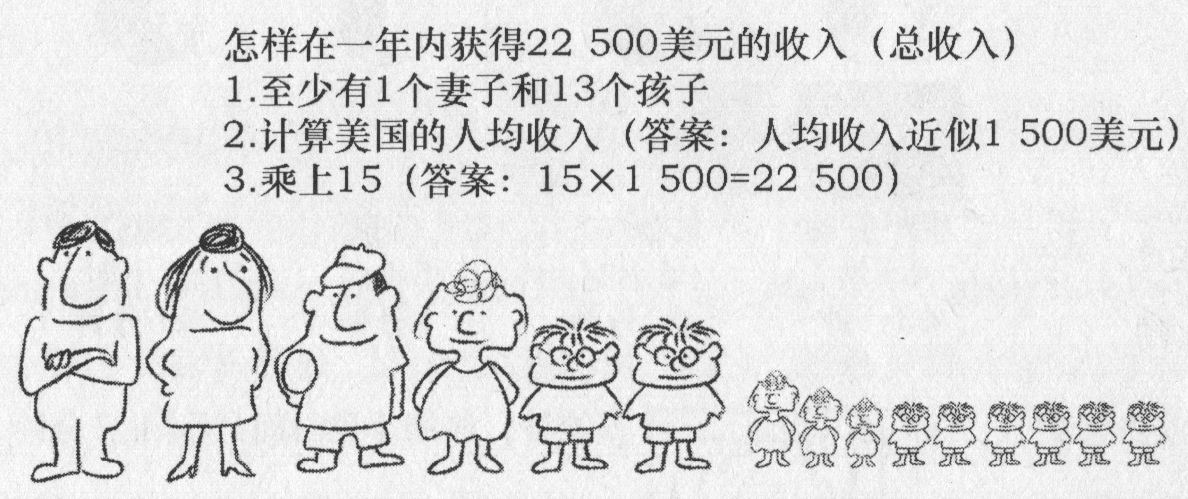
\includegraphics[width=0.9\textwidth]{c6.income.01.png}
  \end{figure}
\end{frame}

\begin{frame}
  \frametitle{拓展 | 不可忽视的权重}
  \begin{figure}
    \centering
    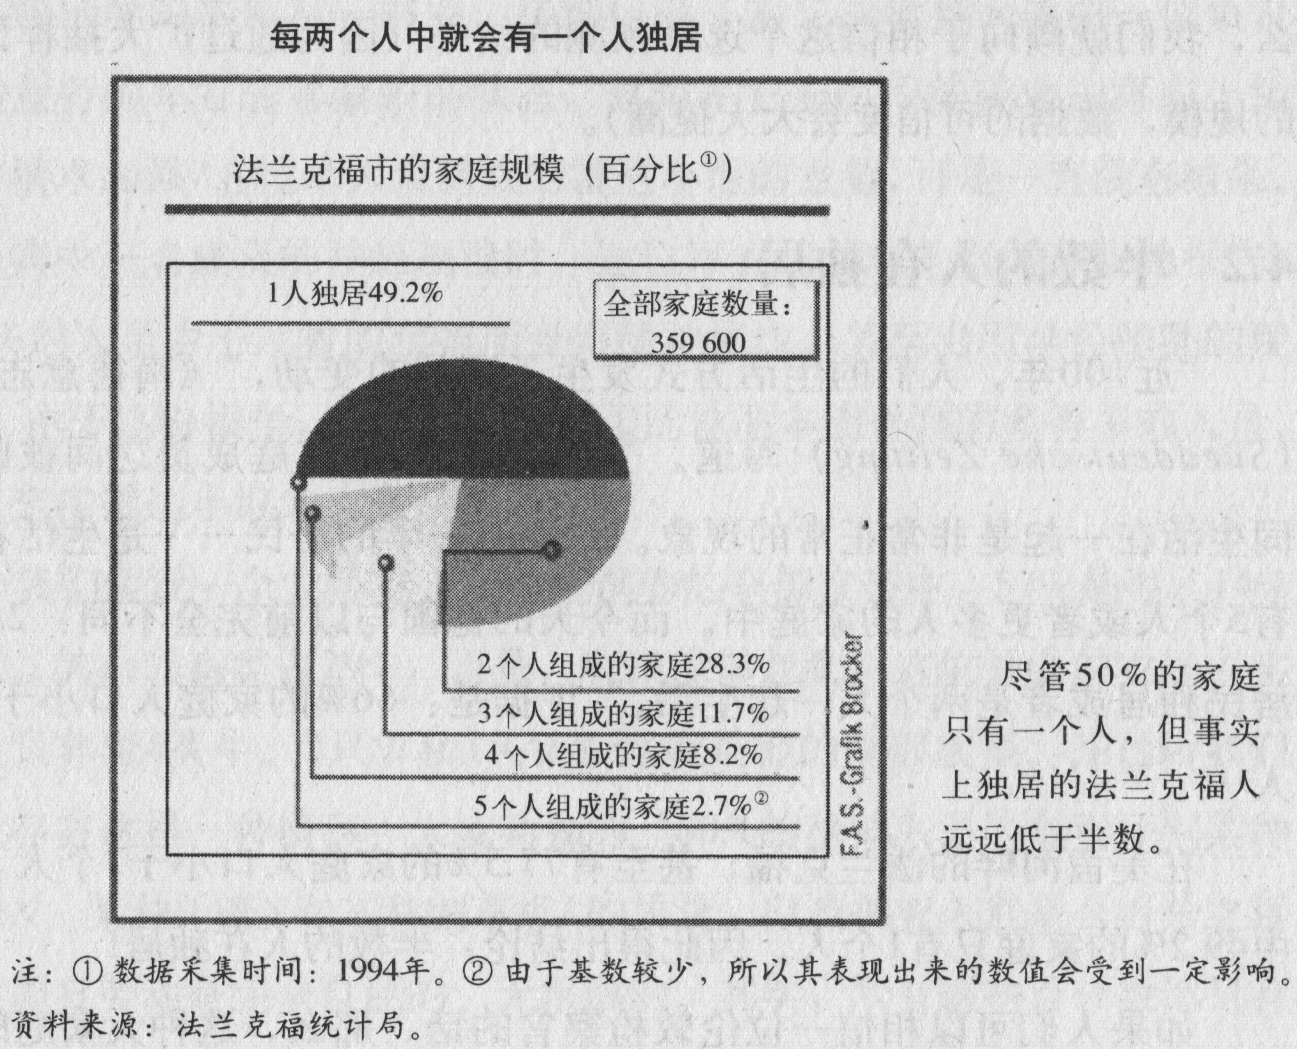
\includegraphics[width=0.8\textwidth]{c6.alone.01.png}
  \end{figure}
\end{frame}

\begin{frame}
  \frametitle{拓展 | 数字越精确结论越不可靠}
  \begin{figure}
    \centering
    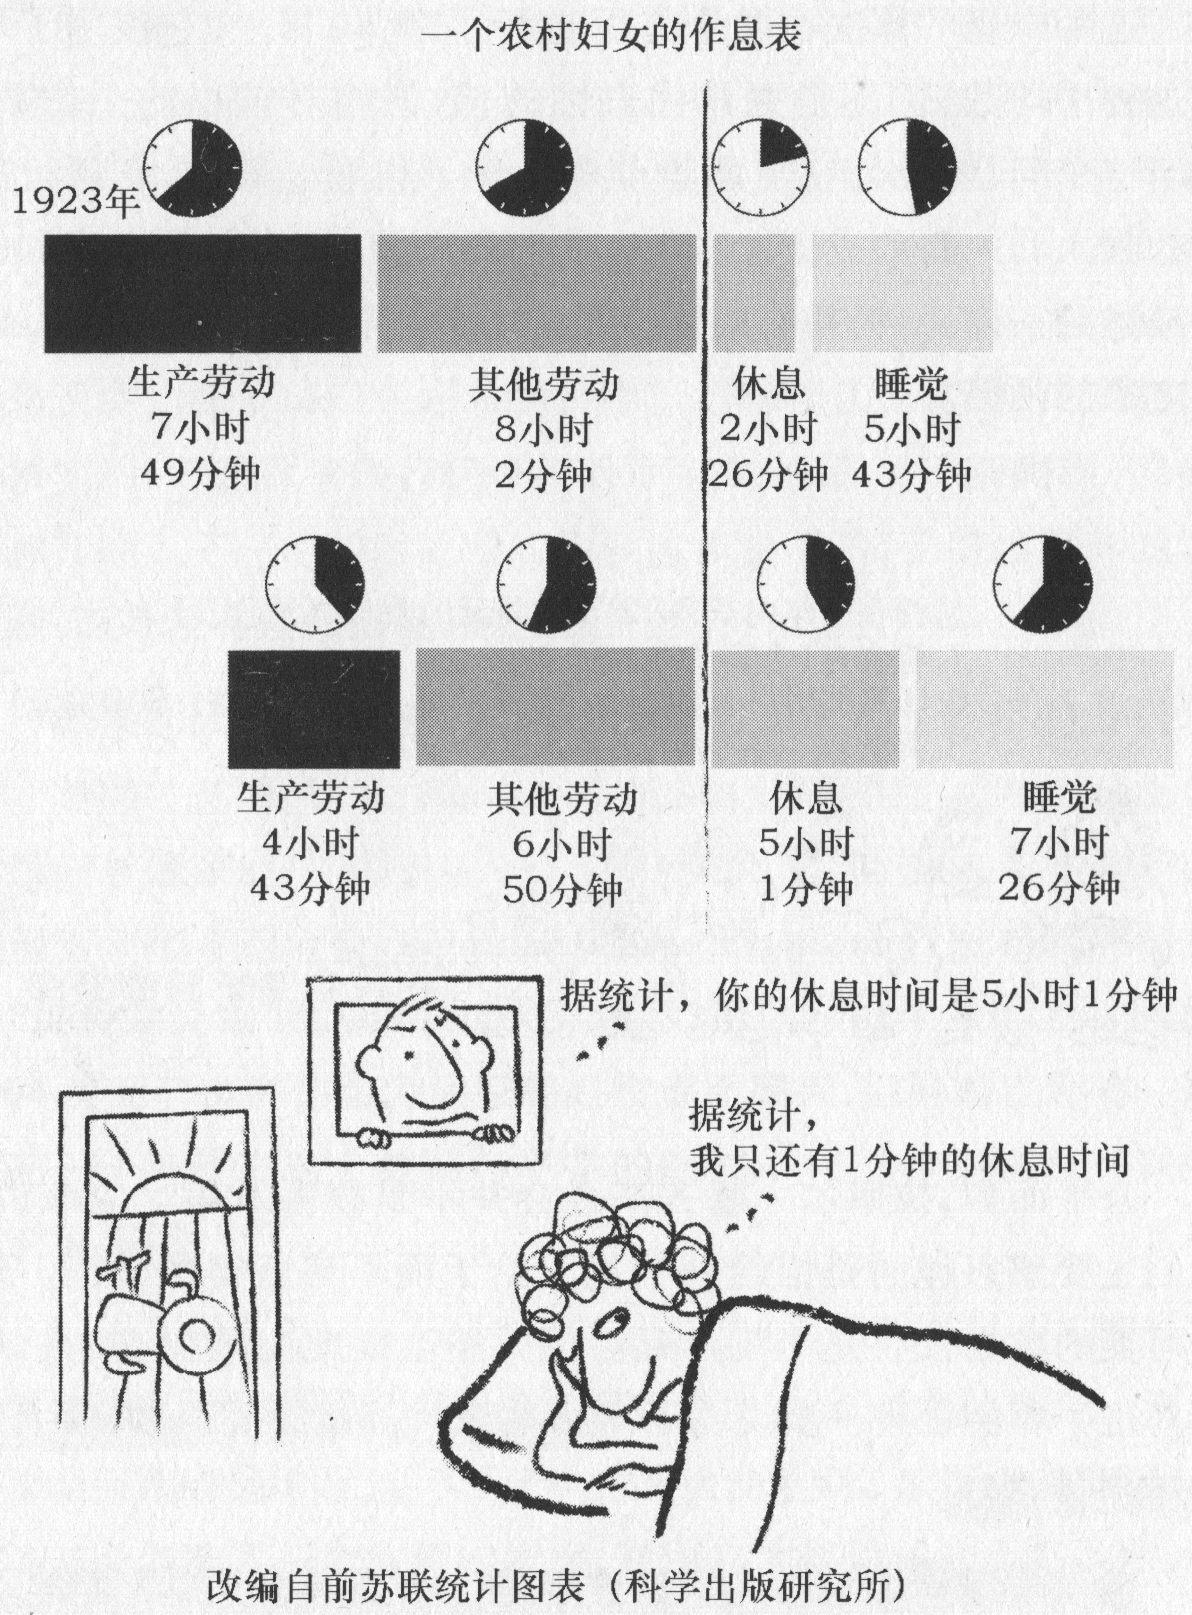
\includegraphics[width=0.45\textwidth]{c6.sleep.01.png}
  \end{figure}
\end{frame}

\begin{frame}
  \frametitle{拓展 | 数字越精确结论越不可靠}
  \begin{figure}
    \centering
    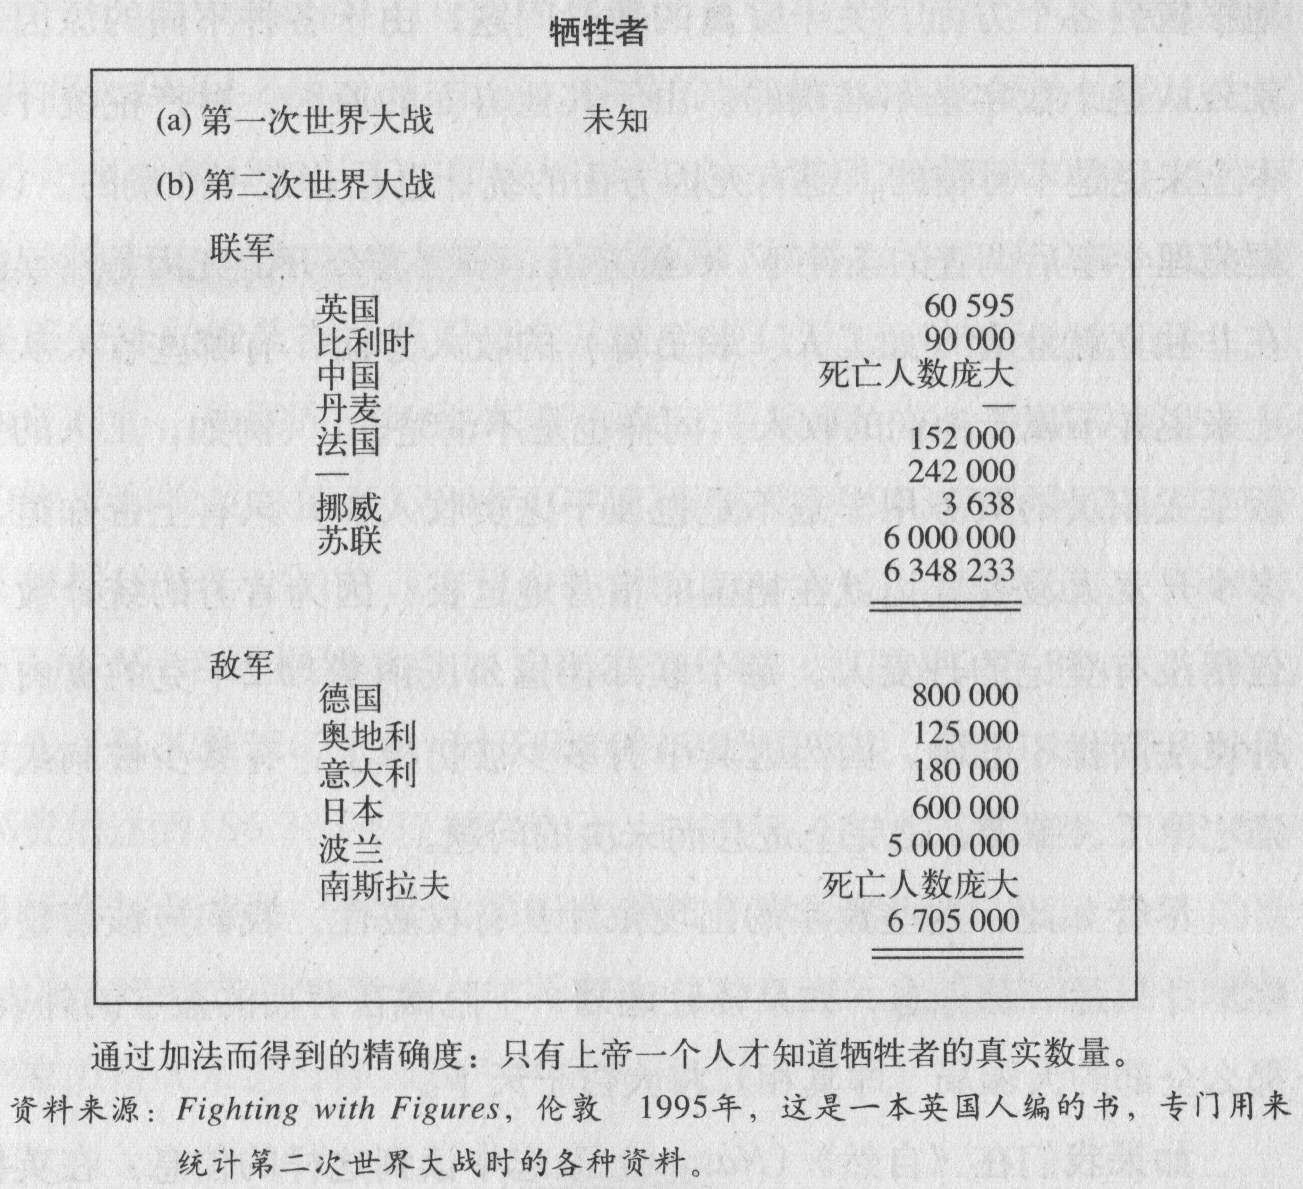
\includegraphics[width=0.7\textwidth]{c6.war.01.png}
  \end{figure}
\end{frame}

\begin{frame}
  \frametitle{拓展 | 变换基数操纵百分比}
  \begin{figure}
    \centering
    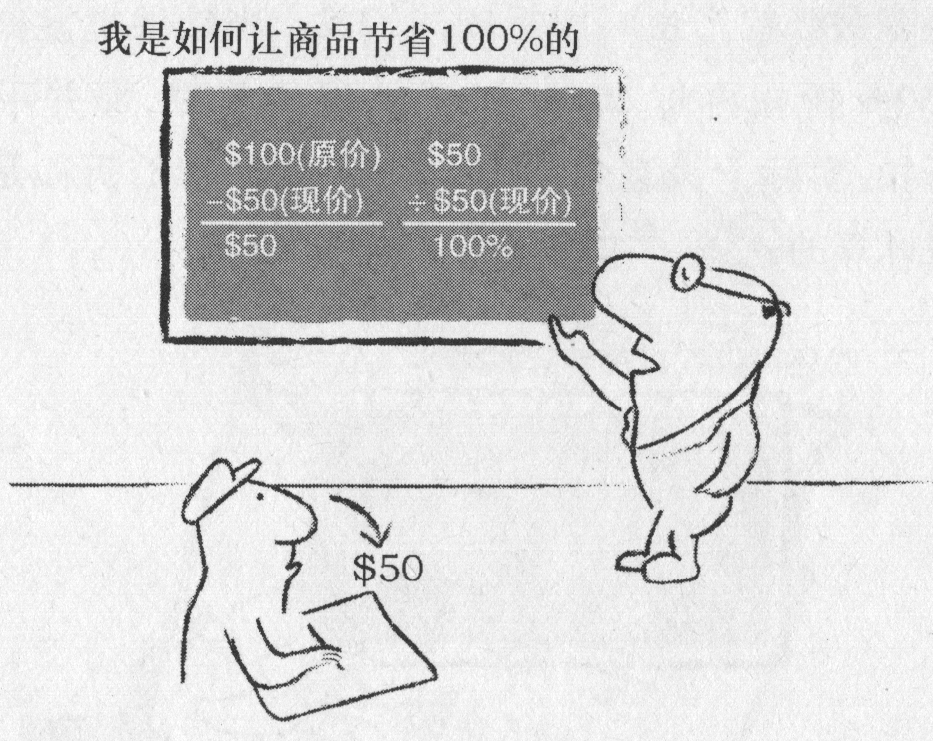
\includegraphics[width=0.4\textwidth]{c6.sale.01.png}\quad
    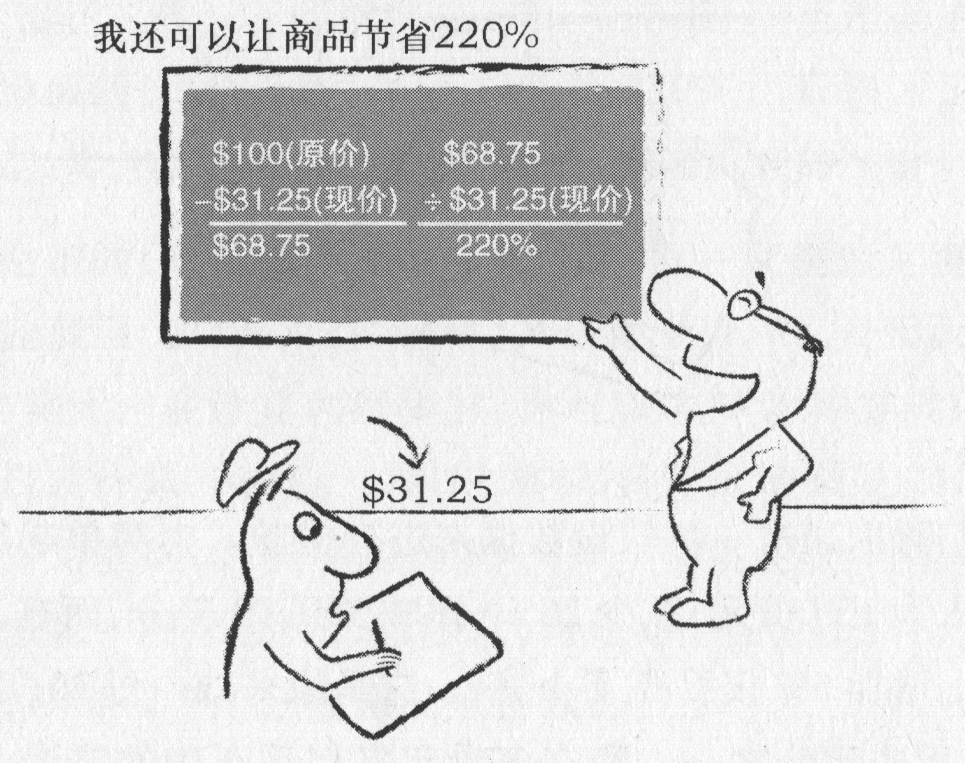
\includegraphics[width=0.4\textwidth]{c6.sale.02.png}
  \end{figure}
\end{frame}

\begin{frame}
  \frametitle{拓展 | 不同的基期不同的结论}
  \begin{block}{问题}
让我们假设去年一夸脱牛奶值10美分,一条面包10美分。今年牛奶的价格降至5美分,而面包的价格升至20美分。现在你想证明什么呢?物价指数上升?物价指数下降?还是根本没有变化?
  \end{block}
  \begin{figure}
    \centering
    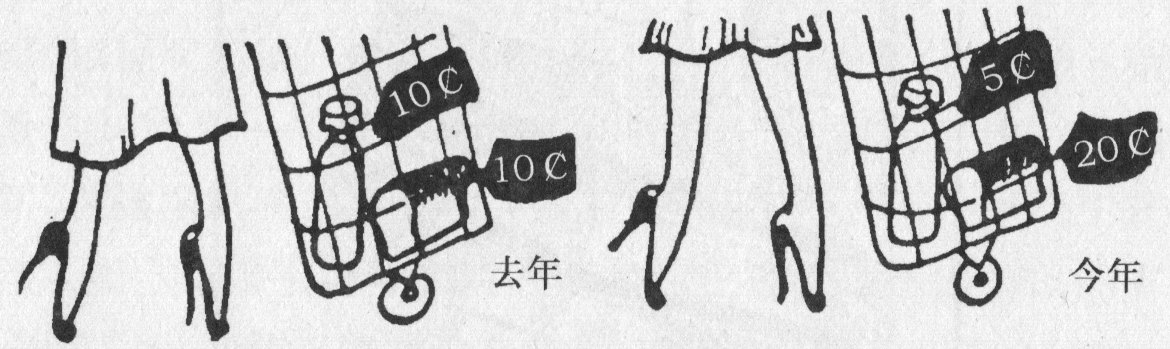
\includegraphics[width=0.9\textwidth]{c6.price.01.png}
  \end{figure}
\end{frame}

\begin{frame}
  \frametitle{拓展 | 不同的基期不同的结论}
  \begin{block}{价格上涨}
 选择去年作为基期,也就是说,以去年的价格为100\%。既然牛奶的价格降低一半(即50\%),而且面包的价格是去年的2倍(即200\%),将50\%与200\%进行平均得125\%,与去年相比,今年的价格上涨了25\%。
  \end{block}
  \begin{figure}
    \centering
    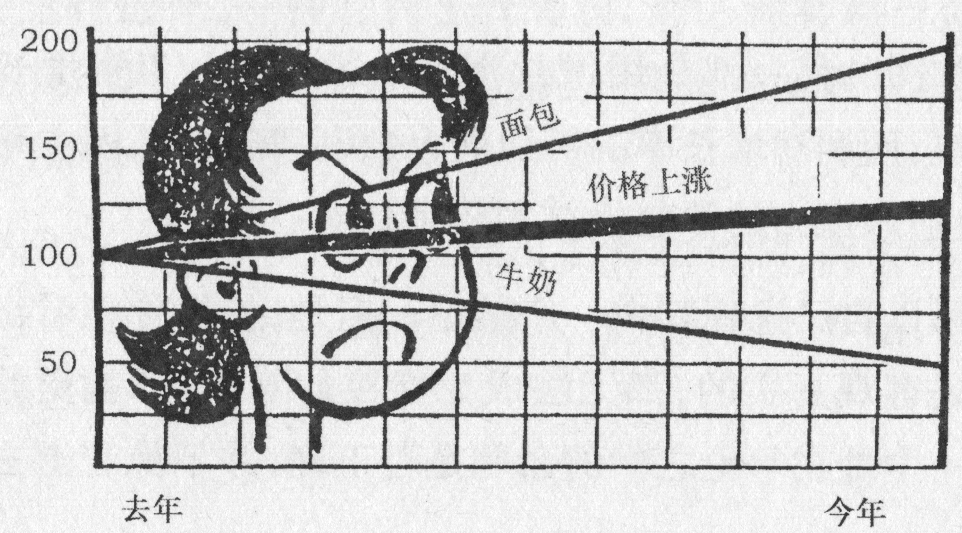
\includegraphics[width=0.7\textwidth]{c6.price.02.png}
  \end{figure}
\end{frame}

\begin{frame}
  \frametitle{拓展 | 不同的基期不同的结论}
  \begin{block}{价格下降}
 以今年的价格为基期。去年牛奶的价格是今年的200\%,而面包的价格是今年的50\%,平均数又是125\%,也就是说,去年的价格比今年的高25\%,今年的价格下降了。
  \end{block}
  \begin{figure}
    \centering
    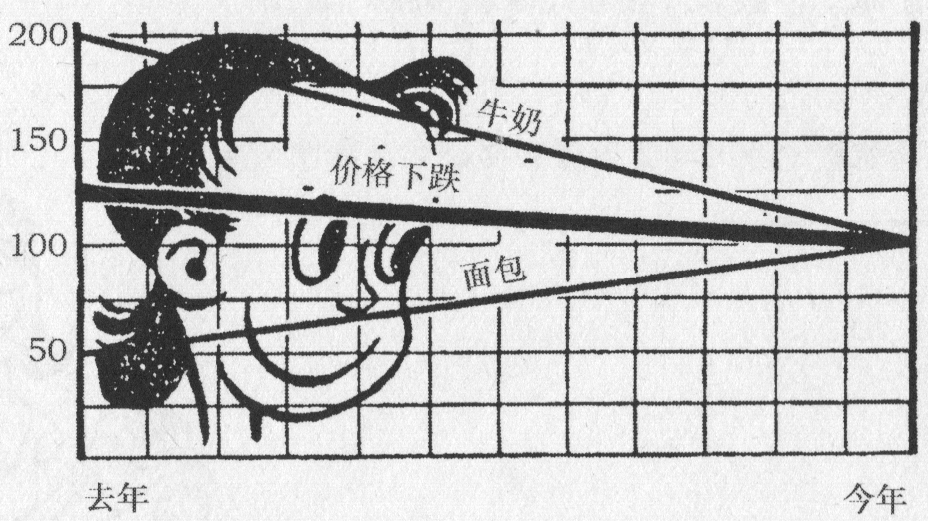
\includegraphics[width=0.7\textwidth]{c6.price.03.png}
  \end{figure}
\end{frame}

\begin{frame}
  \frametitle{拓展 | 不同的基期不同的结论}
  \begin{block}{价格不变}
    如果你想证明价格没有发生变化,试试使用几何平均数,这时你可以随意选择基期。几何平均数不同于算术平均数或者均值,但它也是合理的计算方法,而且在某些情况下它是一种最有效的方法。计算3个数的几何平均数,只需将3个数相乘,开3次方根;4个数的几何平均数,开4次方根,以此类推。\\
    \vspace{0.5em}
  以去年为基期为例,也就是说,去年每种商品的价格都看成100\%,将两个100\%相乘再开平方根,得到100\%,这是去年价格指数的几何平均数。今年牛奶是去年的50\%,面包是去年的200\%,50\%乘以200\%得10000\%,再开平方根得100\%。价格没升也没降。
  \end{block}
\end{frame}

\begin{frame}
  \frametitle{拓展 | 将一些看似能直接相加却不能这样操作的事情加在一起}
  \begin{block}{不需要上学}
一年365天,减去三分之一即122天作为休息时间,再减去约45天作为一日三个小时的进餐时间,余下的198天中再扣除90天度暑假,21天过圣诞节和万圣节。这时余下的时间连过星期六和星期天都不够。
  \end{block}
  \pause
  \begin{block}{一年只工作一天}
    我向老板请一天假,老板推心置腹地说:“你想请一天假?看看你在向公司要求什么——一年里有365天你可以工作。一年52个星期,你已经每星期休息2天,共104天,剩下261天工作。你每天有16小时不在工作,去掉174天,剩下87天。每天你至少花30分钟时间上网,加起来每年23天,剩下64天。每天午饭时间你花掉1小时,又用掉46天,还有18天。通常你每年请2天病假,这样你的工作时间只有16天。每年有5个节假日公司休息不上班,你只干11天。每年公司还慷慨地给你10天假期,算下来你就工作1天,而你TMD还要请这一天假?”
  \end{block}
\end{frame}

\begin{frame}
  \frametitle{拓展 | 将一些看似能直接相加却不能这样操作的事情加在一起}
  \begin{figure}
    \centering
    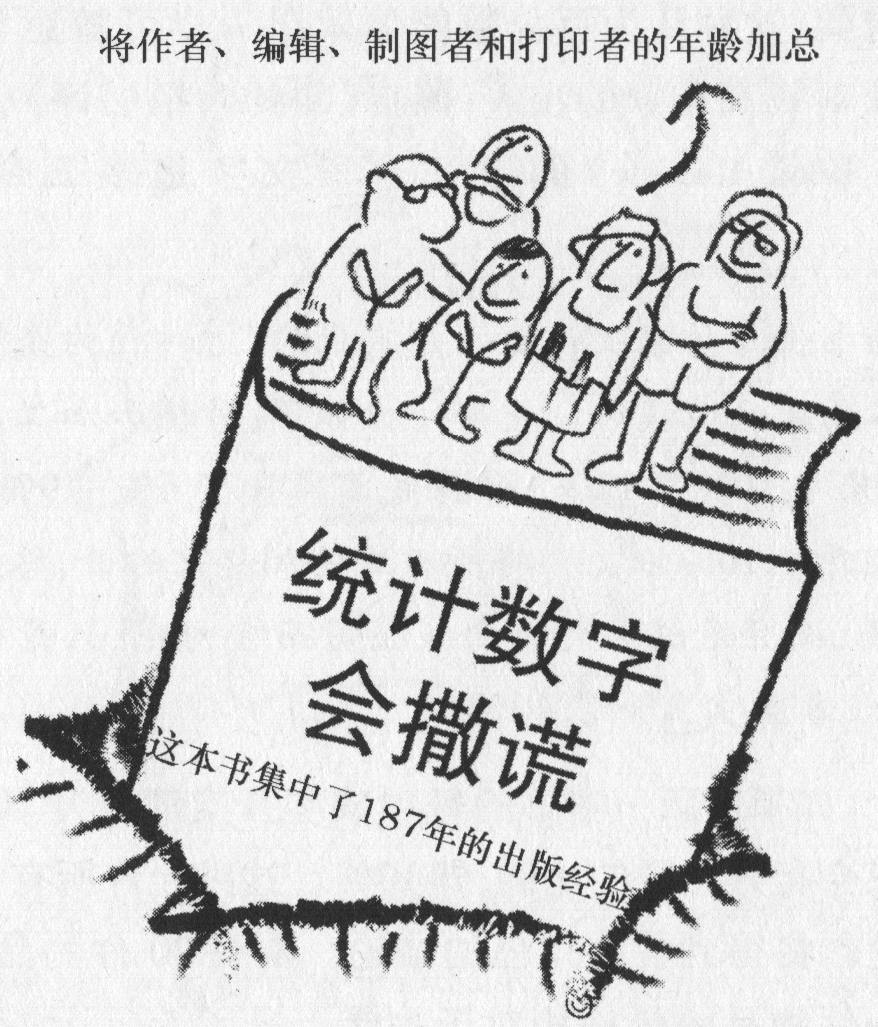
\includegraphics[width=0.5\textwidth]{c6.year.01.png}
  \end{figure}
\end{frame}

\begin{frame}
  \frametitle{拓展 | 将一些看似能直接相加却不能这样操作的事情加在一起}
  加起来200岁的乐队,只组合一年就散伙,却拯救了整个华语乐坛!
  \vspace{-0.5em}
  \begin{figure}
    \centering
    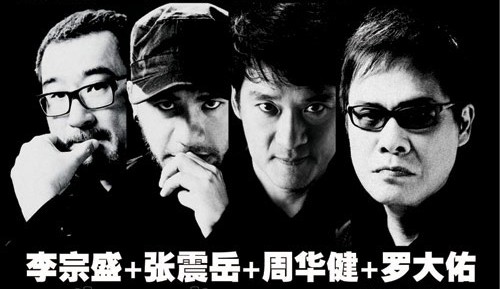
\includegraphics[width=0.9\textwidth]{c6.music.01.jpg}
  \end{figure}
\end{frame}

\begin{frame}
  \frametitle{拓展 | 好“小”的1000万英镑}
  \begin{block}{振兴教育}
    2007年1月,英国政府大肆宣布将加拨1000万英镑的预算,“振兴小学的歌唱与音乐教育”。1000万英镑,看起来好像很大,但这个数字应该附加下列说明:全英有大约1000万名学童,几乎有一半都在念小学,将1000万英镑平均分配给500万个小学生之后,这笔预算到底可以振兴出什么结果?
  \end{block}
  \pause
  \begin{block}{托儿所}
    \begin{itemize}
      \item 5年内花费3亿英镑新增100万间托儿所,这笔钱够不够?
      \item 你找得到一周费用只有1.15英镑的托儿所吗?
    \end{itemize}
  \end{block}
  \pause
  \begin{block}{支付宝红包}
    \begin{itemize}
      \item (2017年)1.68亿人瓜分2亿五福红包——人均1.2元!
      \item (2018年)支付宝集五福全民瓜分5亿红包——2.51亿人/人均1.988元!
    \end{itemize}
  \end{block}
\end{frame}

\section{如何反驳统计资料}
\begin{frame}
  \frametitle{反驳 | 原则}
  \begin{block}{\alert{反驳统计资料}}
    怎样凭双眼就能识破虚假的统计资料,并揭开它的老底;同样重要的是,如何在这一大片充满了欺骗性的数据海洋中找出可靠有用的资料。\\
    \vspace{0.5em}
    你所接触到的统计资料,它们并非都要经受化学分析或者实验室的鉴定才能辨别真伪。但至少你可以提5个简单的问题,在寻找这些问题答案的同时,你将避免接受一些不真实的资料。
    \begin{enumerate}
      \item 谁说的?——寻找偏差(有意识的偏差和无意识的偏差)
      \item 他是如何知道的?——样本是否有偏,数值是否足够大,观察值是否足够多
      \item 遗漏了什么?——包含多少观测值,没有比较,仅给出百分数,巧妙选择基期,遗漏引起变化的原因
      \item 是否有人偷换了概念?——定义方式的改变,偷梁换柱的比较
      \item 这个资料有意义吗?——让人印象深刻的精确数据,不加控制的外推法
    \end{enumerate}
  \end{block}
\end{frame}

\begin{frame}
  \frametitle{反驳 | 数目有多大?}
  \begin{block}{把它个人化}
  太过专注于数字的“大”,往往只会造成混淆视听的效果,除非这刚好是使用这些数字的人想要达到的目标,但又往往不是,反而变成大家一再落入的陷阱。所以,在看到数字时,最重要、简单,却也最少人问起的问题,就是“这个数字大不大?”\\
  \vspace{0.5em}
  每当数字的大小,超过日常应用的熟悉范围,我们就经常会忘记以人类尺度来看待这些天文数字。然而,\alert{人类尺度是让数字变得有意义的最佳工具},也是我们每个人生下来都具备的尺度,运用起来一点也不困难。\\
  \vspace{0.5em}
  \alert{让数字变得有意义的最佳工具,就是以人类尺度来看。}
  \end{block}
\end{frame}

\begin{frame}
  \frametitle{反驳 | 数目有多大? | 实例}
  \begin{columns}
    \column{0.6\textwidth}
  \begin{block}{阅读量}
    大学4年,借阅400本书(确切数字为476册)。
  \end{block}
  \pause
  \pause
  \begin{block}{“科研人才”}
    5年发表40余篇科研论文!——灌水!
  \end{block}
  \pause
  \begin{block}{学科评估}
    2017年,天津财经大学,5名评估专家,5天的时间,“评阅”4000多份毕业论文!(工作到晚上10点,给准备夜宵,……)
  \end{block}
    \column{0.38\textwidth}
    \begin{figure}
      \centering
      \visible<2->{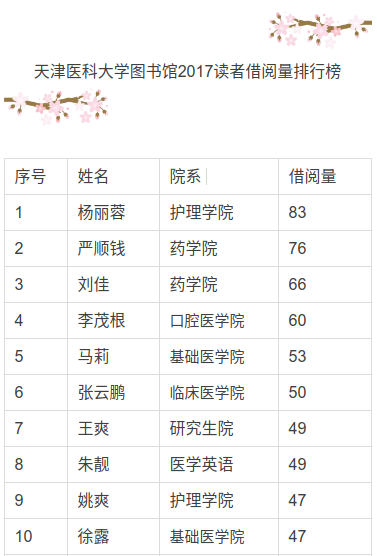
\includegraphics[width=0.9\textwidth]{c6.book.2017.png}}
    \end{figure}
  \end{columns}
\end{frame}

\section{大数据时代的谎言}
\begin{frame}
  \frametitle{大数据 | 骗人?}
  \begin{block}{疑问}
    大数据通过综合数据精密计算得出的结果,怎么会涉及骗人的问题呢?
  \end{block}
  \pause
  \begin{block}{答案}
    看似无稽之谈,但真正的答案是:\alert{会}。
  \end{block}
  \pause
  \begin{block}{定义}
    骗人:给人提供错误的结果或给人带来误导。
  \end{block}
  \pause
  \begin{block}{原因}
    数据来源、分析过程、人的因素都可能带来骗人的效果。
  \end{block}
\end{frame}

\begin{frame}
  \frametitle{大数据 | 数据可视化}
  \begin{block}{引言}
    俗话说一图值千言,数据可视化在数据分析中占有举足轻重的地位,而数据可视化也是“骗人”的重灾区。
  \end{block}
  \vspace{-0.5em}
  \pause
  \begin{block}{骗术}
    \begin{itemize}
      \item 更改坐标轴:有时候是有意的(比如说需要强调自己的某一个看法),有时候是无意的(比如说 Excel 会自动调整)。
      \item 累积分布图:看历年数据趋势的时候,很多时候是既可以看每年的单独分布,也可以看累积分布的,比如说销量、利润等等。有时候碰上今年的销量或者利润不如去年,如果看逐年销量或者利润,则很容易看到下降的趋势。若改成累积分布图,下降的趋势就很容易被抹去了。
      \item 颠倒黑白:虽然说同样的数据可以有不同的解读,可以有不同风格的分析方法,然而有一些基本的套路还是要遵守的,比如说饼图(pie chart)用百分比的时候加起来总和为100\%,纵轴往上为正,往下为负。
    \end{itemize}
  \end{block}
\end{frame}

\begin{frame}
  \frametitle{大数据 | 可视化 | 更改坐标轴 | 投球速度}
  \begin{figure}
    \centering
    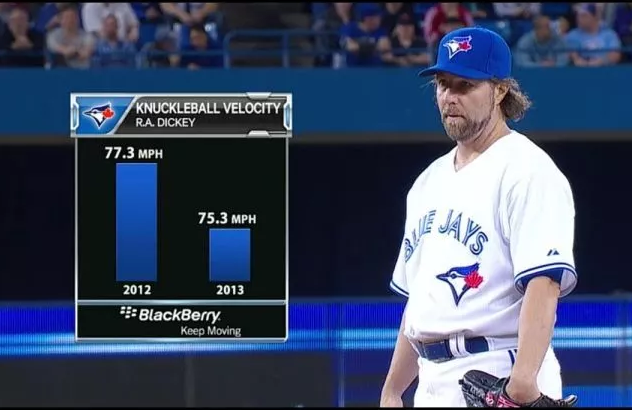
\includegraphics[width=0.9\textwidth]{c6.bigdata.ball.png}
  \end{figure}
\end{frame}

\begin{frame}
  \frametitle{大数据 | 可视化 | 更改坐标轴 | GDP趋势图}
  \begin{figure}
    \centering
    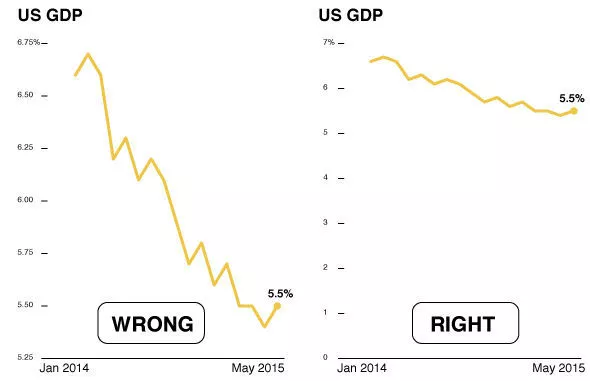
\includegraphics[width=0.9\textwidth]{c6.bigdata.gdp.png}
  \end{figure}
\end{frame}

\begin{frame}
  \frametitle{大数据 | 可视化 | 更改坐标轴 | 胜率对比}
  \begin{figure}
    \centering
    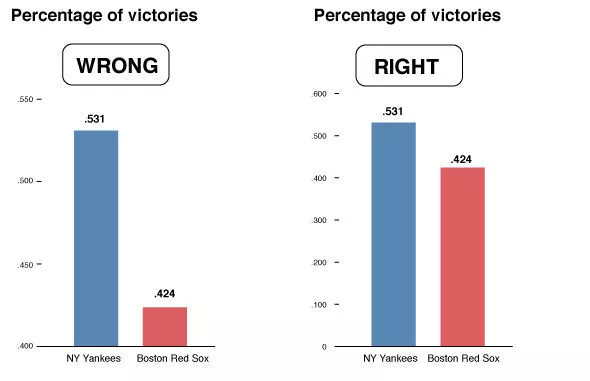
\includegraphics[width=0.9\textwidth]{c6.bigdata.vs.png}
  \end{figure}
\end{frame}

\begin{frame}
  \frametitle{大数据 | 可视化 | 累积分布图 | iPhone销量}
  \begin{figure}
    \centering
    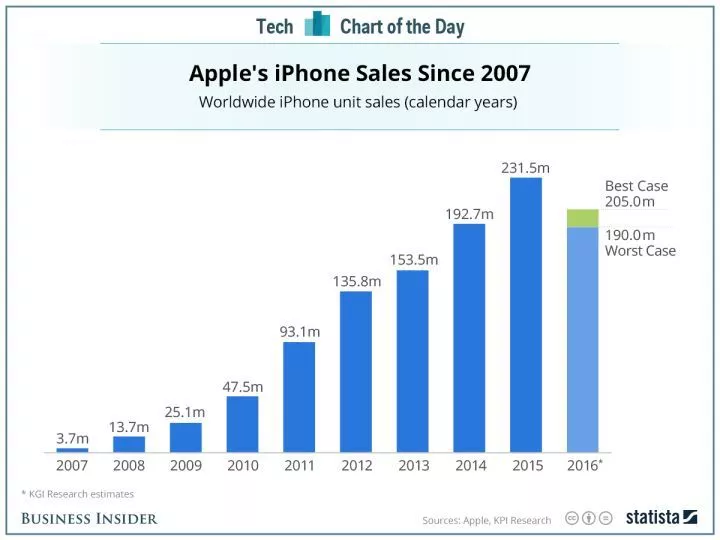
\includegraphics[width=0.43\textwidth]{c6.bigdata.iphone.01.png}
    \visible<2->{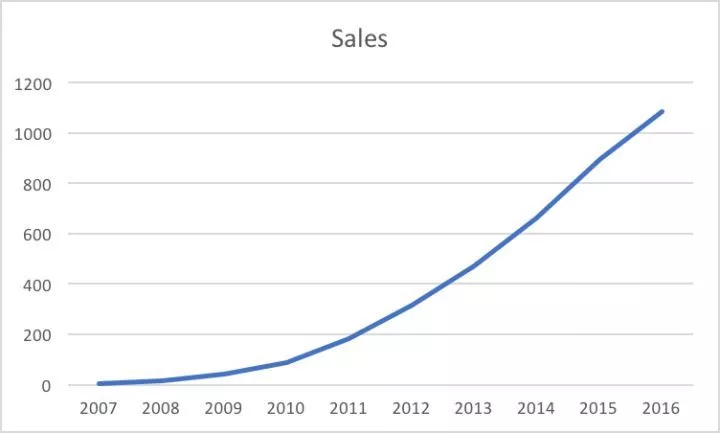
\includegraphics[width=0.55\textwidth]{c6.bigdata.iphone.02.png}}
  \end{figure}
\end{frame}

\begin{frame}
  \frametitle{大数据 | 可视化 | 颠倒黑白 | 美国佛罗里达州通过城堡法之后的命案数}
  \begin{figure}
    \centering
    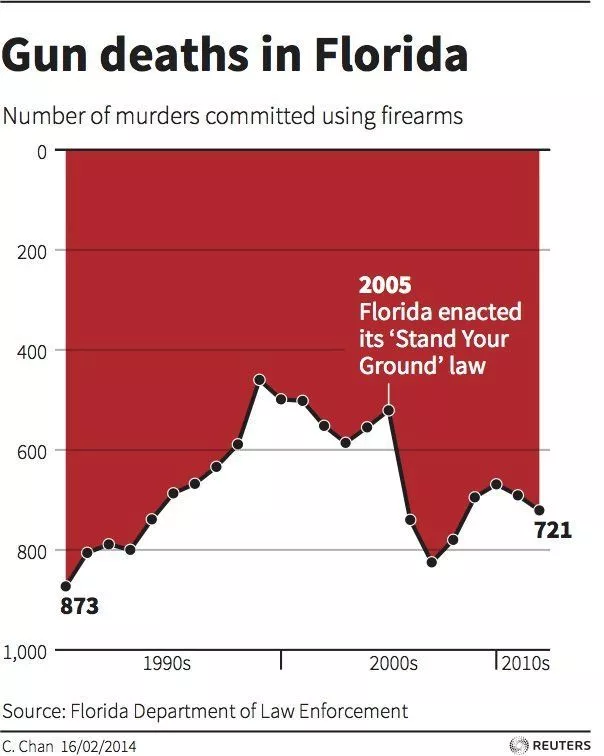
\includegraphics[width=0.5\textwidth]{c6.bigdata.death.png}
  \end{figure}
\end{frame}

\begin{frame}
  \frametitle{大数据 | 错把相关当因果}
  \begin{block}{普林斯顿的研究}
    2013年,一项来自普林斯顿的研究通过对比`MySpace'关键词搜索量和MySpace的发展趋势的相关性,再联系以`Facebook'为关键词的搜索趋势,最后得出结论到2015-2017年之间,Facebook将会失去至少8亿用户。
  \end{block}
  \pause
  \begin{block}{Facebook的反击}
    Facebook的数据科学家Mike Develin利用论文里的方法展开反击,半开玩笑半认真的得出结论,到2021年,普林斯顿将会一个学生都没有了。而更为恐怖的是,利用相同的研究方法,到2060年,地球的空气将不复存在。
  \end{block}
\end{frame}

\begin{frame}
  \frametitle{大数据 | 中国人才流失严重}
  \begin{figure}
    \centering
    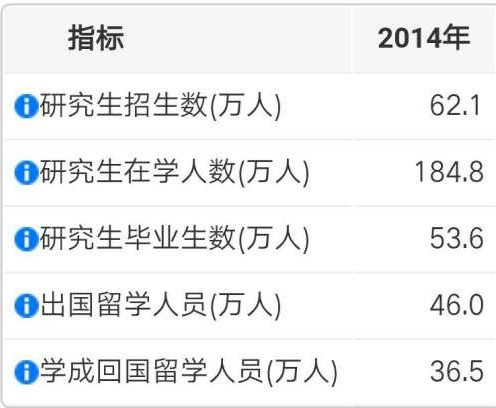
\includegraphics[width=0.45\textwidth]{c6.bigdata.student.01.jpg}
    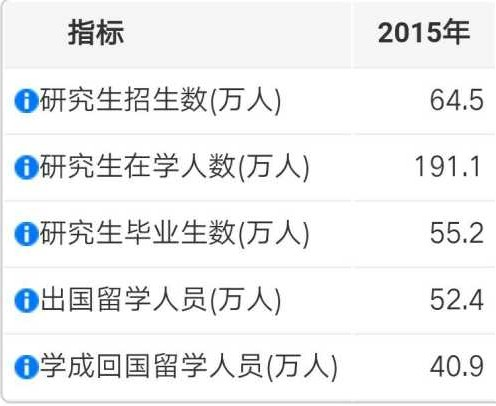
\includegraphics[width=0.45\textwidth]{c6.bigdata.student.02.jpg}
  \end{figure}
  \begin{block}{报道}
    截至2012年底,大陆累计出国留学人数达到264万,留学回国人员仅为109万人——出、归“赤字”超过150万人。到2013年,中国人才流失量居世界首位。
  \end{block}
\end{frame}

\begin{frame}
  \frametitle{大数据 | 中国人才流失严重 | 解析}
  \begin{block}{解析}
    \begin{itemize}
      \item 出国后当年立即回国的有几人?——用当年的回国人数和出国人数计算出来的所谓“归国率”合理吗?
      \item 选择性偏差:大部分不打算回国的留学生,统计局是不会把他们算进这组统计数据中的。国家统计的这个数字,很有可能大部分是在国家留学管理机构注册挂号,准备毕业或工作后回国发展的人,还有很多是通过官方基金资助短期出国做博士后、访问学者的人员。
      \item 何为人才?——出国的不一定是精英。不回来的也不一定是精英。现在出国早就无法等同于高素质,无数的水项目基本等同于高端深度旅游。
      \item 人才的效力有多大?——有时候一个人能顶三个,有时候三个顶不上一个。
    \end{itemize}
  \end{block}
\end{frame}

\section{实例“演示”}
\begin{frame}
  \frametitle{项目缘起}
  \begin{block}{现象}
    班级前几名基本上都是女生,自习室上自习的也以女生居多。
  \end{block}
  \vspace{-0.5em}
  \pause
  \begin{block}{假设}
    女生比男生更加勤奋好学。
  \end{block}
  \pause
  \begin{block}{实验设计}
    \begin{enumerate}[<+->]
      \item 以天津医科大学学生为研究对象
      \item 以暑期留校的学生为样本
      \item 以早晨食堂就餐的学生人数比例进行统计分析
    \end{enumerate}
  \end{block}
  \vspace{-0.5em}
  \pause
  \begin{block}{实验操作}
    2017年暑假的某一天早上7:30,在学校汇贤阁,统计当时食堂内的人数:总人数为20人,其中男生5人,女生15人。得出结论:女生比男生更勤奋好学。
  \end{block}
\end{frame}

\begin{frame}
  \frametitle{设计缺陷}
  \begin{block}{实验设计中可能存在的问题}
    \begin{itemize}
      \item 天津医科大学:男女人数对等吗?——男生、女生的总人数比例。
      \item 暑假留校:哪些学生更倾向于留校?——学生=本科生+研究生。
      \item 汇贤阁:该食堂的代表性如何?——与男女宿舍的距离,男女生对该食堂的偏好。
      \item 早上7:30:时间节点和还是时间段?——男生女生的起床时间。
      \item 食堂与学习:起得早、吃得早不等同于学习勤奋。
      \item ……
    \end{itemize}
  \end{block}
\end{frame}

\section{寄语}
\begin{frame}
  \frametitle{你的世界别人不懂}
  \begin{figure}
    \centering
    
\includegraphics[width=0.5\textwidth]{c6.hope.01.jpg}
  \end{figure}
\end{frame}

\begin{frame}
  \frametitle{你的时区独一无二}
  \begin{figure}
    \centering
    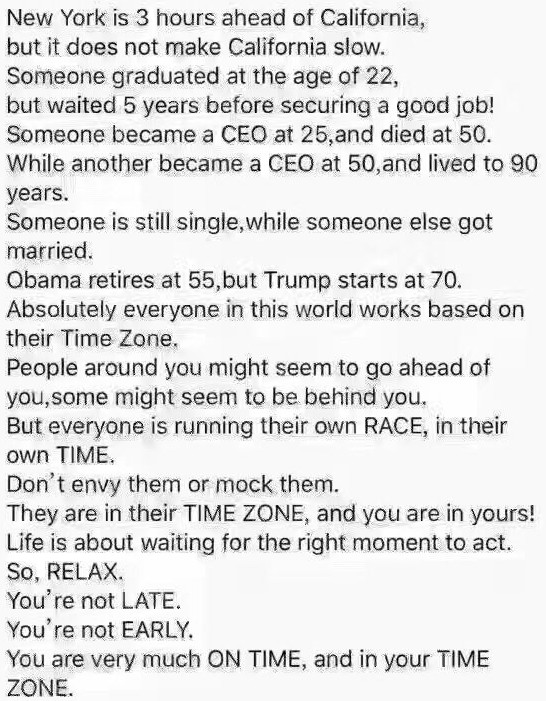
\includegraphics[width=0.5\textwidth]{c6.hope.02.jpg}
  \end{figure}
\end{frame}

\begin{frame}
  \frametitle{你的时区独一无二}
  \begin{block}{时区(1/2)}
纽约时间比加州时间早三个小时,New York is 3 hours ahead of California,\\
但加州时间并没有变慢。but it does not make California slow.\\
有人22岁就毕业了,Someone graduated at the age of 22,\\
但等了五年才找到稳定的工作!but waited 5 years before securing a good job!\\
有人25岁就当上CEO,却在50岁去世。Someone became a CEO at 25, and died at 50.\\
也有人迟到50岁才当上CEO,然后活到90岁。While another became a CEO at 50, and lived to 90 years.\\
有人单身,同时也有人已婚。Someone is still single, while someone else got married.\\
奥巴马55岁就退休,川普70岁才开始当总统。Obama retires at 55, but Trump starts at 70.\\
  \end{block}
\end{frame}

\begin{frame}
  \frametitle{你的时区独一无二}
  \begin{block}{时区(2/2)}
    {\small
世上每个人本来就有自己的发展时区。Absolutely everyone in this world works based on their Time Zone.\\
身边有些人看似走在你前面,也有人看似走在你后面。People around you might seem to go ahead of you, some might seem to be behind you.\\
但其实每个人在自己的时区有自己的步程。But everyone is running their own RACE, in their own TIME.\\
不用嫉妒或嘲笑他们。Don't envy them or mock them.\\
他们都在自己的时区里,你也是!They are in their TIME ZONE, and you are in yours!\\
生命就是等待正确的行动时机。Life is about waiting for the right moment to act.\\
所以,放轻松。So, RELAX.\\
你没有落后。You're not LATE.\\
你没有领先。You're not EARLY.\\
在你自己的时区里,一切安排都准时。You are very much ON TIME, and in your TIME ZONE.
}
  \end{block}
\end{frame}




\section*{Acknowledgements}
\begin{frame}
  \frametitle{Powered by}
  \begin{center}
    
\includegraphics[width=9cm]{power.png}
  \end{center}
\end{frame}

\end{document}

